\section{基線長安定化のための能動防振}
\subsection{従来の能動防振}
Pre-Isolatorの目的はステージを慣性系に対して静止させることである。したがってFeedBackで用いるセンサーには慣性センサーを用いなければならない。しかし図\ref{img:img_seismo_vs_lvdt}が示すように一般的に慣性センサーは低周波で地面振動よりもノイズが大きいため、ループゲインを低周波で大きくすることができず、DC位置を制御することができない。

一方で共振器長制御のためには、ステージの位置制御をしなければならない。そのため低周波ではローカルな変位センサーをつかって、地面の揺れに追従するようにしている。このように慣性センサーと変位センサーをあわせたセンサーのことを super sensor と呼ぶ\cite{hua2005low}。低周波でノイズが大きくなる慣性センサーには high-pass フィルターを、変位センサーには同じカットオフ周波数のlow-pass フィルターをかけている。これらフィルターは相補フィルターと呼ばれており以下のような関係式で結ばれる。
\begin{eqnarray}\label{eq:eq01}
  L(\omega) + H(\omega) = 1
\end{eqnarray}  
ここで、$L(\omega),\,L(\omega)$はそれぞれlow-passフィルターとhigh-passフィルターである。このような super sensor を用いて、高周波では慣性系に、低周波では地面に対してFeedBack制御をおこなっている。。

\begin{figure}[H]
  \begin{center}
    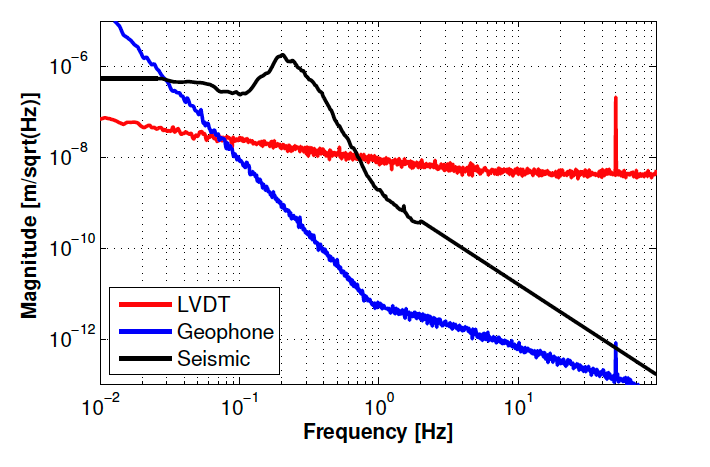
\includegraphics[width=10.0cm]{../arm_length_compensation_system/img_seismo_vs_lvdt.png}
  \end{center}
  \caption{地面振動とセンサーノイズの比較。黒線は地面振動。赤線はLVDT、青線はGeophoneのセンサーノイズを変位に換算したものである。30mHzいかでは地面振動$x_0$よりもGeophoneはノイズが大きい。参考文献\cite{sekiguchiD2016}のFig5.6から転載。}
  \label{img:img_seismo_vs_lvdt}
\end{figure}

\begin{figure}[H]
  \begin{center}
    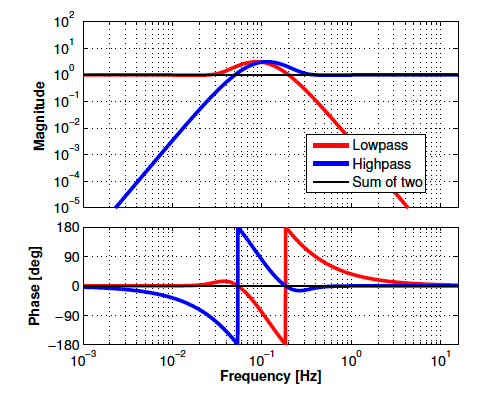
\includegraphics[width=10.0cm]{../arm_length_compensation_system/img_pi_blending.png}
  \end{center}
  \caption{Blendingフィルター。0.1Hzにカットオフ周波数をもつ相補フィルター。
    図\ref{img:img_seismo_vs_lvdt}によれば、0.1HzでGeophoneのノイズがLVDTよりも大きくなるので、0.1Hzにカットオフを持たせなければならない。したがってローパスはLVDTにハイパスはGeophoneにかけている。参考文献\cite{sekiguchiD2016}のFig5.8から転載。}
  \label{img:img_pi_blending}
\end{figure}

\begin{figure}[H]
  \begin{center}
    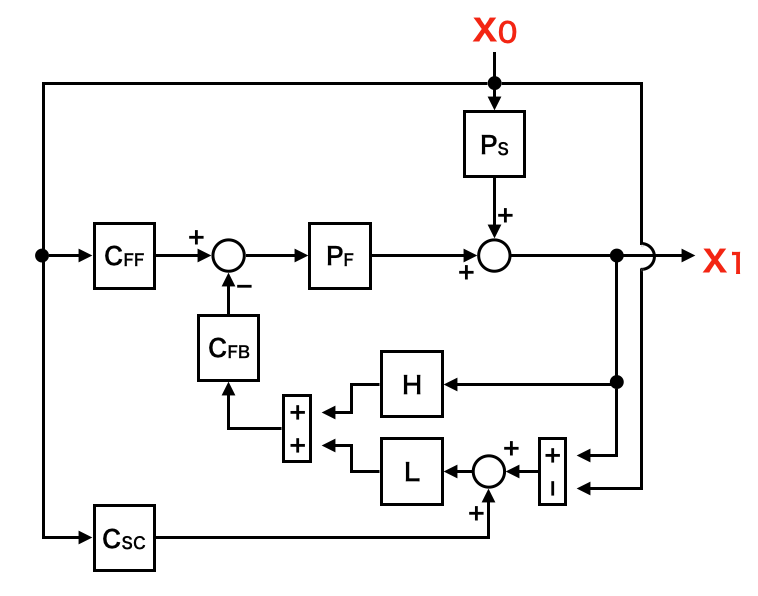
\includegraphics[width=10.0cm]{../arm_length_compensation_system/img_2dof_pi.png}
  \end{center}
  \caption{LIGOのPreisolatorで使用している能動防振のブロック図。参考文献\cite{matichard2015seismic}から引用した。ここで、$P_{\mathrm{s}}$は地面振動の変位$x_0$からステージの変位$x_1$への伝達関数である。$C_{\mathrm{fb}},\,C_{\mathrm{ff}},\,C_{\mathrm{sc}}$はそれぞれ feedback、feedforward、sensor correctionの制御フィルターである。さらに$H,\,L$はsuper sensor のための相補フィルターであり、それぞれ慣性センaサーのためのハイパスフィルターと変位センサーのためのローパスフィルターである。$G$はループゲインをあらわしており$G=C_{\mathrm{fb}}P_{\mathrm{f}}$という関係であり、このときの$P_{\mathrm{f}}$はステージのアクチュエータからステージの変位への伝達関数である。}\label{img:img_2dof_pi}
\end{figure}

\begin{figure}[H]
  \begin{center}
    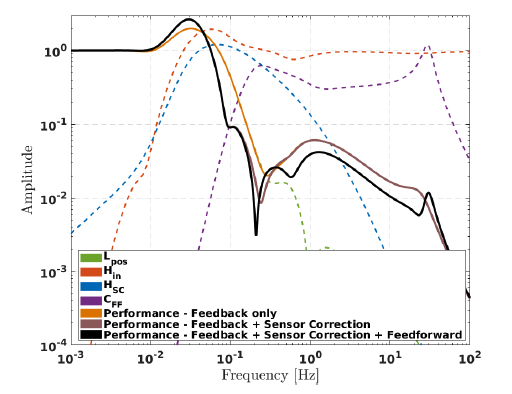
\includegraphics[width=11.0cm]{../arm_length_compensation_system/img_pi_fb_sc_ff.png}
  \end{center}
  \caption{参考文献\cite{biscansD2018}のFig3.13から転載。}
  \label{img:img_pi_fb_sc_ff}
\end{figure}

ところで、変位センサーを使うということはステージが地面と一緒に動くことを意味している。これは比較的小さいスケールの腕共振器であれば、低周波地面振動は同相な地面振動雑音として除去されるので問題となりにくい。しかしkmスケールの腕共振器では、とくにRMSの大きな脈動の帯域では、逆相成分である基線長伸縮は同相成分とくらべて1/4程度にしか低減できない\cite{miyo2018cdmr}。このような問題に対してLIGOではsensor correction と呼ばれるfeed forward 制御を加えた試みをおこなっている\cite{hua2005low}\cite{matichard2015seismic}。


LIGOの sensor correction は feed back ループにある変位センサーから地面振動成分を取り除く方法である。LIGOの能動防振のブロック図を図\ref{img:img_2dof_pi}に示す。\footnote{KAGRAではまだ sensor correction は実装されていない。なのでKAGRAとしては地震計をつかうLIGOを踏襲するよりもGIFの歪み計をつかったほうがいい。現段階だとXアームは歪み計でYアームは地震計にするとか。}この図においてステージの変位$x_1$を地面振動$x_0$で表すと
\begin{eqnarray} \label{eq:eq04}
  x_1 &=& \frac{1}{1+G}\Biggl[(P_{\mathrm{s}}+P_{\mathrm{f}}C_{\mathrm{ff}})x_0\Biggl]
  + \frac{G}{1+G}\Biggl[L(1+C_{\mathrm{sc}})x_0\Biggl]
\end{eqnarray}
になる。ここで低周波の外乱抑制を高めるために式(\ref{eq:eq04})のゲイン$G$を十分に大きくすると式(\ref{eq:eq06}),(\ref{eq:eq07})になる。式(\ref{eq:eq07})によれば、feed back のみの場合、ステージの変位$x_1$はローパスフィルターに沿って地面振動$x_0$を流入させる。しかしsensor correction を加えて$C_{\mathrm{sc}}=-1$となるようにフィルターを作れば地面振動からの寄与を減らすことができる。
\begin{eqnarray}\label{eq:eq06}
  \lim_{G \to \infty} x_{1} &=& L(1+C_{\mathrm{sc}})x_0 \\
  &=&
  %% \begin{cases}\label{eq:eq07}
  %%   \; Lx_{0} & \text{($C_{\mathrm{sc}}=0$)}\\
  %%   \; 0 & \text{($C_{\mathrm{sc}}=-1$)} 
  %% \end{cases}  
\end{eqnarray}

実際に使われている制御フィルターを図\ref{img:img_pi_fb_sc_ff}に示す。sensor correction に使うセンサーには結局のところ慣性センサーをつかうので、フィルター$C_{\mathrm{sc}}$は、super sensor と同様に、低周波で十分に信号を落とさなければならない。また高周波ではコヒーレンスが悪くなるため、実際にはバンドパスフィルターを用いる(図\ref{img:img_pi_fb_sc_ff}の青色の破線)。さらに慣性センサーは低周波では tilt-horizontal coupling と呼ばれる傾斜成分が並進成分にカップルする性質があるため、むやみに低周波成分をパスすることはできない。傾斜成分を補償する別のsensor correction が提案されているが\cite{biscansD2018}、慣性センサーを用いている以上、原理的に低周波帯域での補償には限りがある。

ちなみにsensor correction とは別に高周波帯域のステージの要求値を満たすために、LIGOではもう一つのfeed forward を用意している。それはゲインが小さい帯域で効果を表す。式(\ref{eq:eq08}),(\ref{eq:eq09})にゲインを小さくした場合のステージの変位$x_1$を示す。式(\ref{eq:eq08})によれば、feed back のみの場合は、ステージの変位$x_0$はステージの地面振動応答$P_{\mathrm{s}}$に沿って地面振動を流入させる。このとき、sensor correction と同様に、$C_{\mathrm{ff}}=\frac{P_{\mathrm{s}}}{P_{\mathrm{f}}}$となるようにフィルターをつくれば地面振動からの寄与を減らすことができる。
\begin{eqnarray}\label{eq:eq08}
  \lim_{G \to 0} x_{1} &=& P_{\mathrm{s}}x_0 + P_{\mathrm{f}}C_{\mathrm{ff}}x_0 \\
  &=& 
  %% \begin{cases}\label{eq:eq09}
  %%   \; P_{\mathrm{s}}x_{0} & \text{($C_{\mathrm{ff}}=0$)}\\
  %%   \; 0 & \text{($C_{\mathrm{ff}}=\frac{P_{\mathrm{s}}}{P_{\mathrm{f}}}$)} 
  %% \end{cases}  
\end{eqnarray}


本節では、PreIsolatorは変位センサーを低周波帯域でFeedBackセンサーにつかっていることが原因で、ローカルな地面にステージが追随してしまうことが問題であると述べた。従来の方法ではその解決のためにsensor correction をもちいて、地面振動に追従しないよう制御信号を補正しているが、慣性センサーを使っているのでDCまで補正することができない。

本提案では、視点を変えて、2つの共振器鏡それぞれを慣性系に対して防振するのではなく、エンドテストマス(ETM)をインプットテストマス(ITM)に追従するよう補正をする。つまり、共振器長を一定に保つように補正するという意味である。補正するために用いるセンサーには、腕に併設されたレーザー歪み計をもちいる。これは基線長の伸縮を原理的にはDCまで直接計測することができる。つまりETMとITMの地面振動の変位の差である基線長伸縮$\Delta{L}$
\begin{eqnarray}
  \Delta{L} = x_0-y_0
\end{eqnarray}
を測ることができる。ここで$x_0,\,y_0$はETMXとITMXそれぞれの場所での地面振動である。つまり$x_0$で動いているETMのステージからレーザー歪み計で測った基線長$\Delta{L}$分引いてやれば
\begin{eqnarray}
  test
  %\mathrm{ETM}のステージの変位 = x_0 - \Delta{L} = x_0-(x_0-y_0) = y_0
\end{eqnarray}
のようにETMのステージをITMに追随するように補正することができる。詳細は次節で述べることにする。






\subsection{レーザー歪み計をつかった能動防振}

本提案ではsensor correction のセンサーにレーザー歪み計をつかう。これによりETMのステージの変位をITMの地面振動$y_0$になるよう補正する。つまり図\ref{img:img_pi_etmx}のとおり、$C_{\mathrm{sc}}$に入れる信号には、基線長伸縮である$x_0-y_0$を入れる。$x_0,\, y_0$はそれぞれETMとITMの地面振動を表す。このときのETMのステージの変位$x_1$は

\begin{eqnarray}
  x_1 &=& \frac{1}{1+G}\Biggl[(P_{\mathrm{s}}+P_{\mathrm{f}}C_{\mathrm{ff}})x_0\Biggl]
  + \frac{G}{1+G}\Biggl[L(1+C_{\mathrm{sc}})x_0 - LC_{\mathrm{sc}}y_0\Biggl]
\end{eqnarray}
のとおりになる。ゲイン$G$を十分大きくし$C_{\mathrm{sc}}=-1$となるようにすれば、式(\ref{eq:eq11})のとおり、ETMのステージの変位はITMと一致する。
\begin{eqnarray}\label{eq:eq10}
  \lim_{G \to \infty} x_{1} &=& L\Biggl[x_0+C_{\mathrm{sc}}x_0-C_{\mathrm{sc}}y_0\Biggl] \\
  &=&  
  %% \begin{cases}\label{eq:eq11}
  %%   \; Lx_{0} & \text{($C_{\mathrm{sc}}=0$)} \\
  %%   \; Ly_{0} & \text{($C_{\mathrm{sc}}=-1$)} 
  %% \end{cases}  
\end{eqnarray}

%% レーザー歪み計はDCまで感度があるので低周波まで補正することができる。図\ref{img:img_seismo_vs_gif}によれば、脈動は十分にレーザー歪み計で測定できるので、ローパスフィルターは1Hz付近までカットオフ周波数を大きくすることができる。そうすることで、tilt-horizontal coupling による傾斜成分の混入を低減することができる。つまり、

\begin{figure}[H]
  \begin{center}
    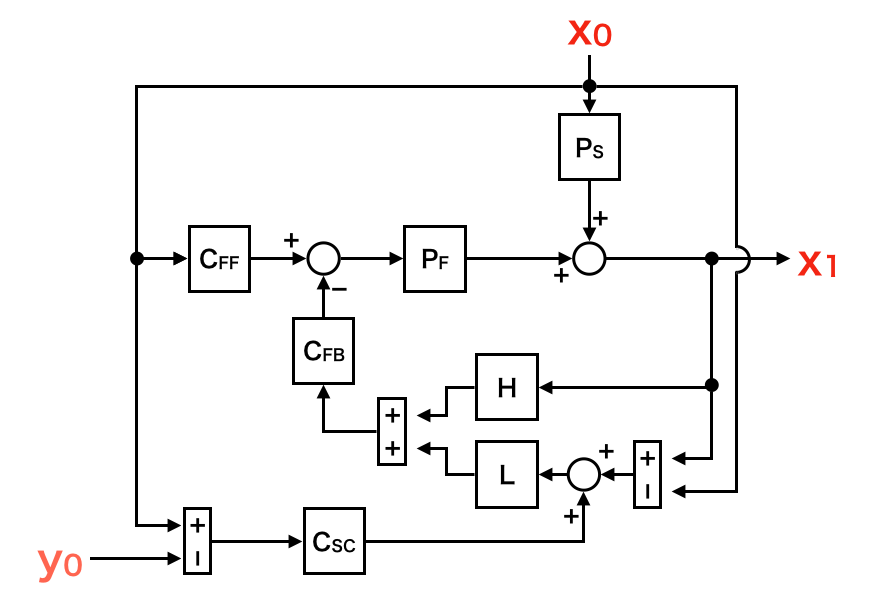
\includegraphics[width=10.0cm]{../arm_length_compensation_system/img_pi_etmx.png}
  \end{center}
  \caption{レーザー歪み計をsensor correction にもちいた能動防振のブロック図。図\ref{img:img_2dof_pi}のsensor correction の信号を$x_0$から$x_0-y_0$に変えた構成。ここで$x_0$はETMXの地面振動で$y_0$はITMXの地面振動である。}\label{img:img_pi_etmx}
\end{figure}


%% \begin{figure}[H]
%%   \begin{center}
%%     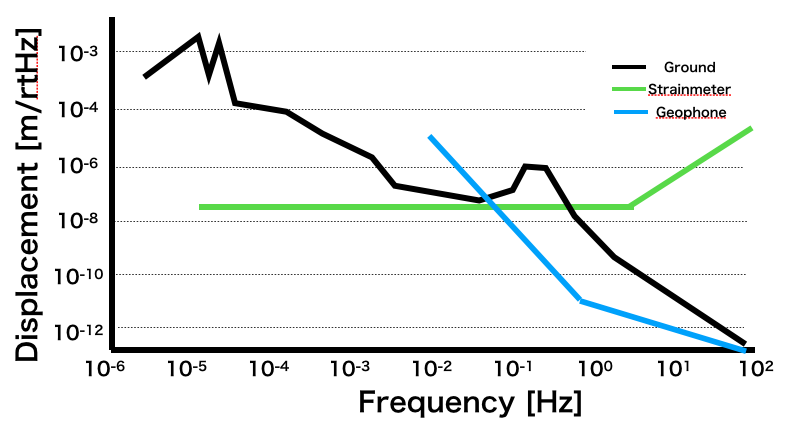
\includegraphics[width=10.0cm]{../arm_length_compensation_system/img_seismo_vs_gif.png}
%%   \end{center}
%%   \caption{レーザー歪み計と慣性センサーのノイズ比較。(実際のデータでグラフを作り直す。歪み計が脈動まで)}\label{img:img_seismo_vs_gif}
%% \end{figure}

%% \begin{figure}[H]
%%   \begin{center}
%%     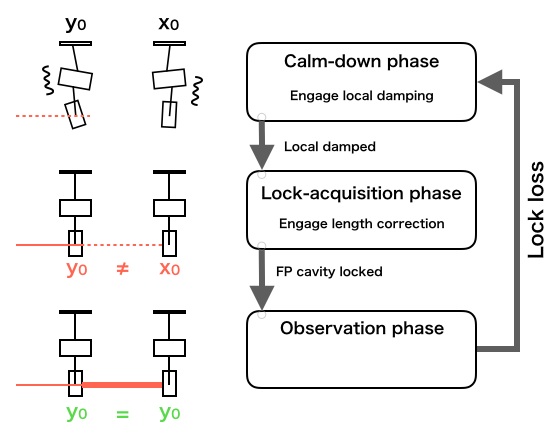
\includegraphics[width=10.0cm]{../arm_length_compensation_system/img_control_transition_diagram.png}
%%   \end{center}
%%   \caption{腕共振器の状態遷移図。}\label{img:img_control_transition_diagram}
%% \end{figure}


%% \subsection{ノイズバジェット}


\appendix
%% \section{2自由度制御}

%% \begin{figure}[H]
%%   \begin{center}
%%     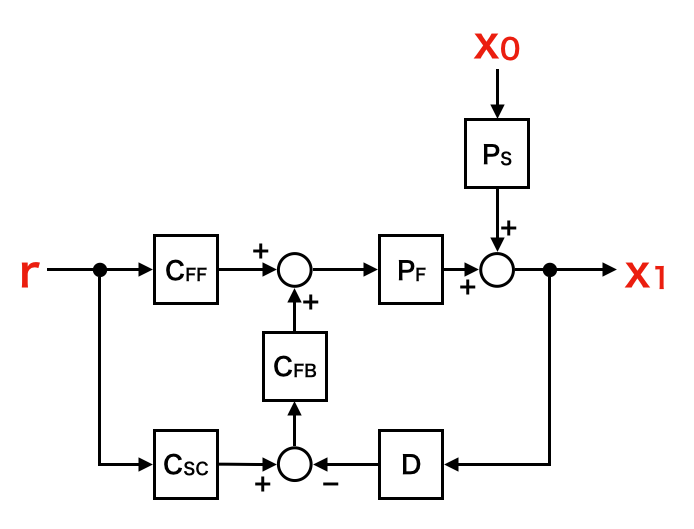
\includegraphics[width=10.0cm]{../arm_length_compensation_system/img_2dof.png}
%%   \end{center}
%%   \caption{}\label{img:img_2dof}
%% \end{figure}

%% 能動防振でつかわれている2自由度制御を説明するよりも先に、2自由度制御のひな形を用いて、2自由度制御の利点である、外乱抑制性能と目標追従性能の両方を向上できることを示しておかなければならない。まずステージの変位$x_1$を目標値$r$と外乱$x_0$で表すと式(\ref{eq:eqA01})のとおりになる。
%% \begin{eqnarray} \label{eq:eqA01}
%%   x_1 &=& \frac{1}{1+G}\Biggl[P_{\mathrm{s}}x_0 + P_{\mathrm{f}}C_{\mathrm{ff}}r\Biggl] + \frac{G}{1+G}\Biggl[\frac{C_{\mathrm{sc}}}{D}\Biggl]r
%% \end{eqnarray}
%% もし$C_{\mathrm{ff}}=1$かつ$C_{\mathrm{sc}}=0$であれば一般的なFeedBack制御になるが、2自由度制御では式(\ref{eq:eqA01})の第2項が加わるおかげで外乱抑制と目的値追従を両方とも良くすることができる。それはつまり外乱抑制をよくするためにGを大きくとると、
%% \begin{eqnarray} \label{eq:eqA02}
%%   \lim_{G \to \infty} x_1 = \frac{C_{SC}}{D}r
%% \end{eqnarray}
%% となり、適当な$C_{\mathrm{sc}}$を選べば、$x_{1}=r$となって、制御後の値$x_{1}$を目標値$r$に一致させることができるためである。

%% \section{式置き場}

%% \begin{eqnarray}
%%   d_1 &=& \frac{1}{1+G}P_{S}d_0 \\
%%   &+& \frac{G}{1+G}\Biggl[L(1-C_{SC})-\frac{C_{FF}+C_{GIF}}{C_{FB}}\Biggl]d_0 \nonumber \\
%%   &-& \frac{G}{1+G}\Biggl[HN_{H} + LN_{SC} + LN_{L} + \frac{C_{FF}}{C_{FB}}N_{FF} + \frac{C_{GIF}}{C_{FB}}N_{GIF} \Biggl] \nonumber
%% \end{eqnarray}

%% \begin{eqnarray}
%%   \lim_{G \to \infty} \langle|d_1|^2\rangle =
%%   \biggl\langle\biggl|[L(1-C_{SC})-\frac{C_{FF}+C_{GIF}}{C_{FB}}]d_0\biggl|^2\biggl\rangle + \langle|N_{\mathrm{all}}|^2 \rangle \\
%% N_{\mathrm{all}} \equiv HN_{H} + LN_{SC} + LN_{L} + \frac{C_{FF}}{C_{FB}}N_{FF} + \frac{C_{GIF}}{C_{FB}}N_{GIF} \nonumber
%% \end{eqnarray}
%% %
%% %
